%
% T�TULO DEL CAP�TULO
%
\chapter[Structure]{
	Structure of a point-based visualizer
	\label{chapter_4}
}

In this chapter, the structure of PCM and ToView is shown. Thus, a high level description of the pipeline is done, which serves as a summary of the analysis phase for this project. The different stages of the pipeline are thoroughly described in the following chapters. Finally, a class diagram depicts the main design aspects of ToView and the updated version of PCM. 

\section[Analysis]{Analysis}

\begin{figure}
        \vspace*{0.5cm}
                \centering
				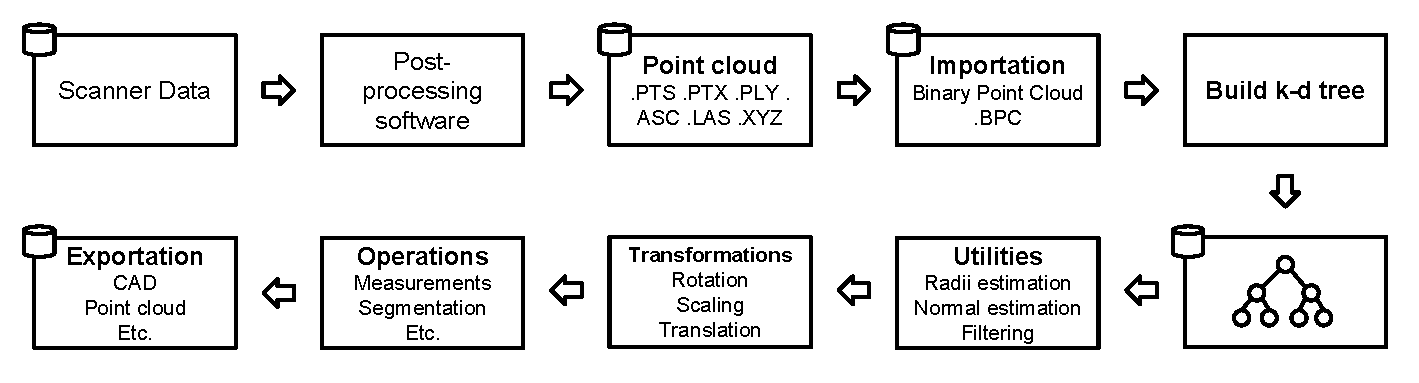
\includegraphics[scale=0.6]{figures/pipeline.pdf}
                \caption[BDE pipeline]{
                        Representation of the usage pipeline of ToView.
                }
                \label{pipeline}
        \vspace*{0.5cm}
\end{figure}

\figurename~\ref{pipeline} depicts the usage pipeline of ToView. To use the system, a series of steps have to be followed. First, the raw LiDAR data is usually processed using software from the manufacturer (unifying scans, calibration, etc.). Once the resulting point cloud from the aforementioned software is available, it will be converted to our point cloud format. 

Next, the k-d tree for accelerating calculations and rendering is created. When the k-d is created and stored in permanent memory, it can be used to estimate radii, normals, apply filters, etc. It can also be used to visualize the point clouds in an efficient way, since we have massive datasets and visualizing them in a naive way is not possible. 

In addition, multiple point clouds can be merged using the visualizer. The user will be able to apply transformations (rotation, scaling and translation) to the individual clouds. This allows the user to for example mix a point cloud that represents a statue with another of its destination, and see in advance how it will look.

ToView can also be used to measure distances in point clouds that were registered with this purpose in mind. Lastly, the visualizer can be used to segment parametric primitives (planes, cylinders and spheres) and export them to a CAD compatible format.        

\section[Design]{Design}
 
ToView is developed following an object oriented approach and using the C{}\verb!++! language \cite{primerplus}. In addition, design patterns have been used as much as possible. The compilers used until now have been Visual C{}\verb!++! in Windows systems, GCC in Linux and Clang in MacOS X. For the creation of multi-platform project files, we have made available a CMake \cite{cmake} makefile for PCM and ToView. For the visualization of the datasets, OpenGL will be used in conjunction with QT. All of these technologies together will allow the user to use the software in the operating system of choice.  

\subsection[Use cases]{Use cases}

In this subsection, the uses of the software package from the user point of view will be detailed. In our system there will be two types of actors, a normal user and a developer. The normal user will use the interface to interact with our software, while the developer will use the library to run its own algorithms to point clouds of arbitrary size. 

We now proceed to detail the use cases presented on \figurename~\ref{use_case_user}:

\begin{figure}[p]
                \centering
                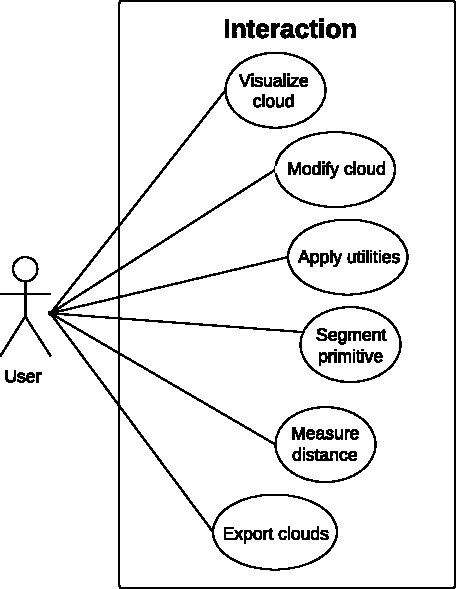
\includegraphics[scale=1.2]{figures/user.pdf}
                \caption[ToView interaction use case diagram]{
                        ToView interation use case diagram.
                }
                \label{use_case_user}
\end{figure}

\newpage

\begin{usecase}

	\addtitle{Use Case 1}{Visualize cloud} 
	
	%Scope: the system under design
	\addfield{Scope:}{System-wide}
	
	%Primary Actor: Calls on the system to deliver its services.
	\addfield{Primary Actor:}{User}
	
	%Preconditions: What must be true on start and worth telling the reader?
	\addfield{Preconditions:}{}
	%when multiple
	%\additemizedfield{Preconditions:}{} 
	
	%Postconditions: What must be true on successful completion and worth telling the reader
	\addfield{Postconditions:}{}
	%when multiple
	%\additemizedfield{Preconditions:}{}
	
	%Main Success Scenario: A typical, unconditional happy path scenario of success.
	\addscenario{Main Success Scenario:}{
		\item User starts ToView
		\item Converts dataset to BPC format
		\item Builds k-d tree
		\item Opens k-d tree folder
		\item Moves around the scene
		\item Closes the visualizer
	}
	
	%Extensions: Alternate scenarios of success or failure.
	\addscenario{Extensions:}{
		\item[3.a] Error building k-d tree:
			\begin{enumerate}
			\item[1.] System shows failure message
			\item[2.] User returns to step 2
			\end{enumerate}
		\item[4.a] No k-d tree present in folder:
			\begin{enumerate}
			\item[1.] System shows failure message
			\item[2.] User returns to step 3
			\end{enumerate}
	}
	
	%Miscellaneous: Such as open issues/questions
	%\addfield{Open Issues:}{}

\end{usecase}

\pagebreak

\begin{usecase}

	\addtitle{Use Case 2}{Modify cloud} 
	
	%Scope: the system under design
	\addfield{Scope:}{System-wide}
	
	%Primary Actor: Calls on the system to deliver its services.
	\addfield{Primary Actor:}{User}
	
	%Preconditions: What must be true on start and worth telling the reader?
	\addfield{Preconditions:}{Having a k-d tree}
	%when multiple
	%\additemizedfield{Preconditions:}{} 
	
	%Postconditions: What must be true on successful completion and worth telling the reader
	\addfield{Postconditions:}{}
	%when multiple
	%\additemizedfield{Preconditions:}{}
	
	%Main Success Scenario: A typical, unconditional happy path scenario of success.
	\addscenario{Main Success Scenario:}{
		\item User starts ToView
		\item Opens k-d tree folder
		\item Chooses operation to perform
		\item The system applies the operation 
		\item[] \textit{The steps 3-4 are repeated for each operation desired}
		\item Closes the visualizer
	}
	
	%Extensions: Alternate scenarios of success or failure.
	\addscenario{Extensions:}{
		\item[2.a] No k-d tree present in folder:
			\begin{enumerate}
			\item[1.] System shows failure message
			\item[2.] User returns to step 1
			\end{enumerate}
	}
	
	%Miscellaneous: Such as open issues/questions
	%\addfield{Open Issues:}{}

\end{usecase}

\pagebreak

\begin{usecase}

	\addtitle{Use Case 3}{Apply utilities} 
	
	%Scope: the system under design
	\addfield{Scope:}{System-wide}
	
	%Primary Actor: Calls on the system to deliver its services.
	\addfield{Primary Actor:}{User}
	
	%Preconditions: What must be true on start and worth telling the reader?
	\addfield{Preconditions:}{Having a k-d tree}
	%when multiple
	%\additemizedfield{Preconditions:}{} 
	
	%Postconditions: What must be true on successful completion and worth telling the reader
	\addfield{Postconditions:}{}
	%when multiple
	%\additemizedfield{Preconditions:}{}
	
	%Main Success Scenario: A typical, unconditional happy path scenario of success.
	\addscenario{Main Success Scenario:}{
		\item User starts ToView
		\item Opens k-d tree folder
		\item Chooses filter, radii or normal estimation 
		\item The system applies the utility 
		\item[] \textit{The steps 3-4 are repeated for each utility}
		\item The system or User saves the changes
		\item User closes the visualizer
	}
	
	%Extensions: Alternate scenarios of success or failure.
	\addscenario{Extensions:}{
		\item[2.a] No k-d tree present in folder:
			\begin{enumerate}
			\item[1.] System shows failure message
			\item[2.] User returns to step 1
			\end{enumerate}
	}
	
	%Miscellaneous: Such as open issues/questions
	%\addfield{Open Issues:}{}

\end{usecase}

\pagebreak

\begin{usecase}

	\addtitle{Use Case 4}{Segment primitive} 
	
	%Scope: the system under design
	\addfield{Scope:}{System-wide}
	
	%Primary Actor: Calls on the system to deliver its services.
	\addfield{Primary Actor:}{User}
	
	%Preconditions: What must be true on start and worth telling the reader?
	\addfield{Preconditions:}{Having a k-d tree}
	%when multiple
	%\additemizedfield{Preconditions:}{} 
	
	%Postconditions: What must be true on successful completion and worth telling the reader
	\addfield{Postconditions:}{}
	%when multiple
	%\additemizedfield{Preconditions:}{}
	
	%Main Success Scenario: A typical, unconditional happy path scenario of success.
	\addscenario{Main Success Scenario:}{
		\item User starts ToView
		\item Opens k-d tree folder
		\item Selects the primitive segmentation settings 
		\item Selects a point in the dataset 
		\item System samples neighborhood
		\item System segments primitive
		\item[] \textit{The steps 3-6 are repeated for each primitive}
		\item User closes the visualizer
	}
	
	%Extensions: Alternate scenarios of success or failure.
	\addscenario{Extensions:}{
		\item[2.a] No k-d tree present in folder:
			\begin{enumerate}
			\item[1.] System shows failure message
			\item[2.] User returns to step 1
			\end{enumerate}
		\item[4.a] No points selected:
			\begin{enumerate}
			\item[1.] System shows failure message
			\item[2.] User returns to step 3
			\end{enumerate}
	}
	
	%Miscellaneous: Such as open issues/questions
	%\addfield{Open Issues:}{}

\end{usecase}

\pagebreak

\begin{usecase}

	\addtitle{Use Case 5}{Measure distance} 
	
	%Scope: the system under design
	\addfield{Scope:}{System-wide}
	
	%Primary Actor: Calls on the system to deliver its services.
	\addfield{Primary Actor:}{User}
	
	%Preconditions: What must be true on start and worth telling the reader?
	\addfield{Preconditions:}{Having a k-d tree}
	%when multiple
	%\additemizedfield{Preconditions:}{} 
	
	%Postconditions: What must be true on successful completion and worth telling the reader
	\addfield{Postconditions:}{}
	%when multiple
	%\additemizedfield{Preconditions:}{}
	
	%Main Success Scenario: A typical, unconditional happy path scenario of success.
	\addscenario{Main Success Scenario:}{
		\item User starts ToView
		\item Opens k-d tree folder
		\item Selects to measure distance
		\item Selects a point in the dataset 
		\item Selects another point
		\item System outputs distance
		\item[] \textit{The steps 3-6 are repeated for each measurement}
		\item User closes the visualizer
	}
	
	%Extensions: Alternate scenarios of success or failure.
	\addscenario{Extensions:}{
		\item[2.a] No k-d tree present in folder:
			\begin{enumerate}
			\item[1.] System shows failure message
			\item[2.] User returns to step 1
			\end{enumerate}
		\item[4-5.a] No points selected:
			\begin{enumerate}
			\item[1.] System shows failure message
			\item[2.] User returns to step 3
			\end{enumerate}
	}
	
	%Miscellaneous: Such as open issues/questions
	%\addfield{Open Issues:}{}

\end{usecase}

\pagebreak

\begin{usecase}

	\addtitle{Use Case 6}{Export data} 
	
	%Scope: the system under design
	\addfield{Scope:}{System-wide}
	
	%Primary Actor: Calls on the system to deliver its services.
	\addfield{Primary Actor:}{User}
	
	%Preconditions: What must be true on start and worth telling the reader?
	\addfield{Preconditions:}{Successful segmentation made}
	%when multiple
	%\additemizedfield{Preconditions:}{} 
	
	%Postconditions: What must be true on successful completion and worth telling the reader
	\addfield{Postconditions:}{}
	%when multiple
	%\additemizedfield{Preconditions:}{}
	
	%Main Success Scenario: A typical, unconditional happy path scenario of success.
	\addscenario{Main Success Scenario:}{
		\item User selects export type
		\item Inputs the output file name
		\item System exports the corresponding data
	}
	
	%Extensions: Alternate scenarios of success or failure.
	\addscenario{Extensions:}{
		\item[2.a] Invalid file name:
			\begin{enumerate}
			\item[1.] System shows failure message
			\item[2.] User returns to step 1
			\end{enumerate}
	}
	
	%Miscellaneous: Such as open issues/questions
	%\addfield{Open Issues:}{}

\end{usecase}

\pagebreak

Next, the use cases on \figurename~\ref{use_case_developer} will be specified:

\begin{figure}[h]
                \centering
                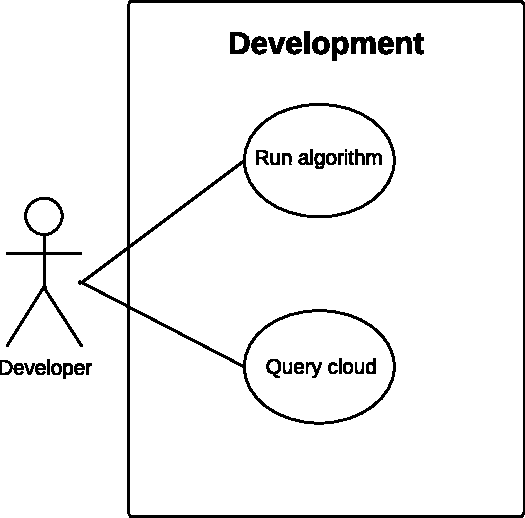
\includegraphics[scale=0.8]{figures/developer.pdf}
                \caption[ToView developer use case diagram]{
                        ToView developer use case diagram.
                }
                \label{use_case_developer}
\end{figure}

\pagebreak

\begin{usecase}

	\addtitle{Use Case 7}{Run algorithm} 
	
	%Scope: the system under design
	\addfield{Scope:}{System-wide}
	
	%Primary Actor: Calls on the system to deliver its services.
	\addfield{Primary Actor:}{Developer}
	
	%Preconditions: What must be true on start and worth telling the reader?
	\addfield{Preconditions:}{}
	%when multiple
	%\additemizedfield{Preconditions:}{} 
	
	%Postconditions: What must be true on successful completion and worth telling the reader
	\addfield{Postconditions:}{}
	%when multiple
	%\additemizedfield{Preconditions:}{}
	
	%Main Success Scenario: A typical, unconditional happy path scenario of success.
	\addscenario{Main Success Scenario:}{
		\item Developer selects algorithm 
		\item Uses PCM's external interface to implement algorithm
		\item Selects precision desired
		\item Converts cloud to .BPC
		\item Creates k-d tree
		\item The system executes the algorithm
		\item The system displays or saves result
	}
	
	%Extensions: Alternate scenarios of success or failure.
	\addscenario{Extensions:}{
		\item[5.a] Error building k-d tree:
			\begin{enumerate}
			\item[1.] System shows failure message
			\item[2.] User returns to step 2
			\end{enumerate}
	}
	
	%Miscellaneous: Such as open issues/questions
	%\addfield{Open Issues:}{}

\end{usecase}

\pagebreak

\begin{usecase}

	\addtitle{Use Case 8}{Query cloud} 
	
	%Scope: the system under design
	\addfield{Scope:}{System-wide}
	
	%Primary Actor: Calls on the system to deliver its services.
	\addfield{Primary Actor:}{Developer}
	
	%Preconditions: What must be true on start and worth telling the reader?
	\addfield{Preconditions:}{Having a k-d tree}
	%when multiple
	%\additemizedfield{Preconditions:}{} 
	
	%Postconditions: What must be true on successful completion and worth telling the reader
	\addfield{Postconditions:}{}
	%when multiple
	%\additemizedfield{Preconditions:}{}
	
	%Main Success Scenario: A typical, unconditional happy path scenario of success.
	\addscenario{Main Success Scenario:}{
		\item Developer selects k-d tree 
		\item Uses PCM's external interface to make a query
		\item The system obtains the requested parts of the cloud
		\item Developer uses the provided information for a certain purpose
	}
	
	%Extensions: Alternate scenarios of success or failure.
	\addscenario{Extensions:}{
		\item[1.a] No k-d tree present in folder:
			\begin{enumerate}
			\item[1.] System shows failure message
			\item[2.] User returns to step 1
			\end{enumerate}
	}
	
	%Miscellaneous: Such as open issues/questions
	%\addfield{Open Issues:}{}

\end{usecase}

\pagebreak

\subsection[Class diagram]{Class diagram}

Now that we have exposed the conceptual approach, we show the class diagram of the engine. It will be further explained in the next chapters.

\begin{figure}[h]
                \centering
                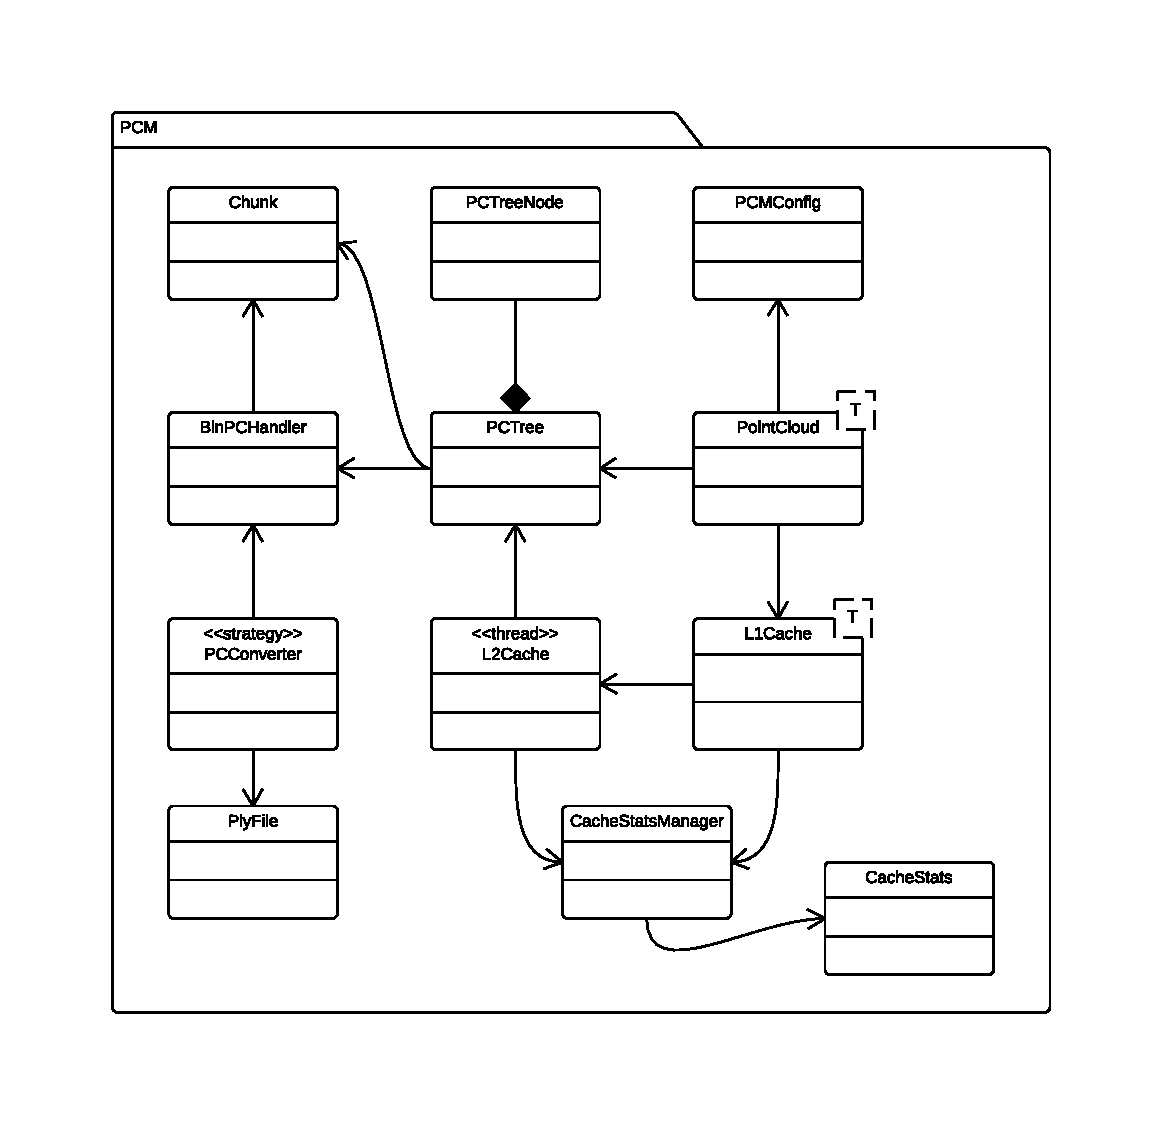
\includegraphics[scale=0.6]{figures/PCM.pdf}
                \caption[PCM class diagram]{
                        PCM class diagram.
                }
                \label{class_dia}
\end{figure}

On one hand we have the library \textbf{PCM} (see \figurename~\ref{class_dia}) that consists of:

\textbf{Chunk} represents the minimum amount of information that will travel across the different levels of memory, that is why its size in bytes will be closely controlled. \textbf{BinPCHandler} is the intermediate compacted format (BPC) in the format conversion process and the spatial structure construction, its objective is representing an arbitrary length array of data that resides in permanent storage. \textbf{PCConverter} is the class in charge of offering a single interface to convert any type of point cloud file.

The spatial structure is represented by \textbf{PCTree}. This class encapsulates two main functionalities, the construction of the chunk database and the multi-resolution tree management and its nodes. \textbf{PCTreeNode} contains information about the nodes that make up the spatial structure. 

Next, the classes associated with memory management will be briefly described. \textbf{L2Cache} is the class responsible of the exchange of data between HDD and RAM. \textbf{L1Cache} is in charge of transferring data between RAM and VRAM. Both classes use \textbf{CacheStatsManager} to keep track of several statistics, like hit rate, miss rate, etc. 

\begin{figure}[h]
                \centering
                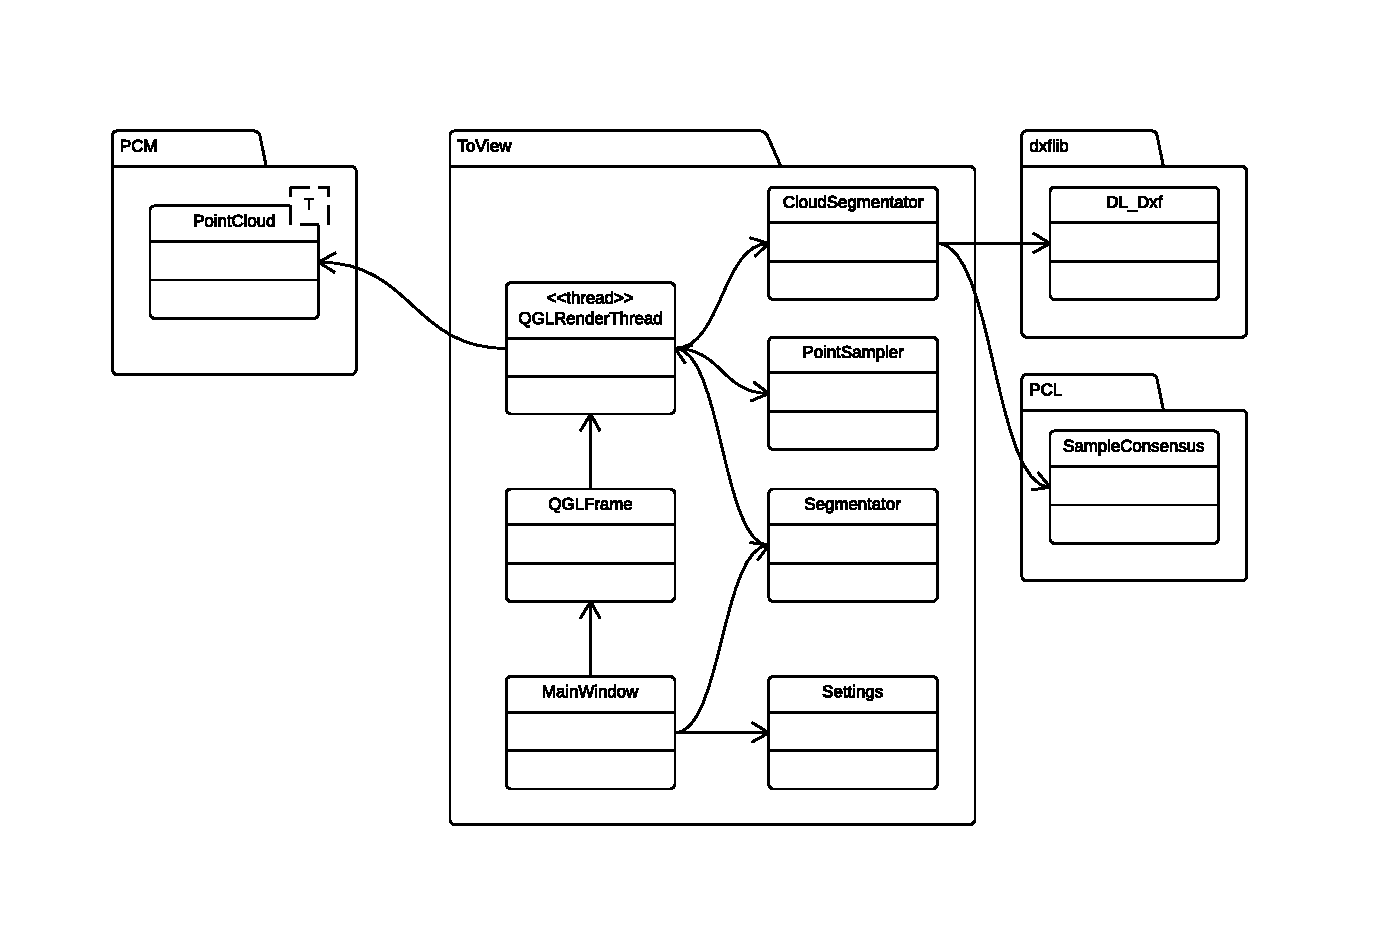
\includegraphics[scale=0.6]{figures/ToView.pdf}
                \caption[ToView class diagram]{
                        ToView class diagram.
                }
                \label{class_dia_tov}
\end{figure}

\textbf{PointCloud} represents a complete dataset and is the external interface of the library. It will allow the user to request information about the dataset, to load a region, apply a certain operation, etc. This class is accompanied by \textbf{PCMConfig} that stores several information about the characteristics of the point cloud.

On the other hand we have the visualizer \textbf{ToView} (see \figurename~\ref{class_dia_tov}) that is formed by:

\textbf{MainWindow} is the class that represents the main window of the visualizer. It contains the navigation menus and the widget in which the rendering will be done. The \textbf{Settings} class is where all the information related to the configuration of ToView will be stored and provides the interface to modify it. \textbf{Segmentator} is in charge of providing the interface for the user to be able to control and use the segmentation feature of the visualizer and modify its settings.

\textbf{QGLFrame} is responsible for creating the OpenGL context. It is also in charge of processing mouse and keyboard events. The rendering thread \textbf{QGLRenderThread} will also be launched from this class. As the name implies, this is the class that renders the point clouds. 

\textbf{PointSampler} will allow the user to sample points from a point cloud to be able to measure distances or segment primitives later. \textbf{CloudSegmentator} is the class responsible for segmenting and exporting the supported primitives.     




